%!TEX program = xelatex
\documentclass[11pt,class=book]{standalone}
%\usepackage[utf8]{inputenc}
\usepackage[french]{babel}
\usepackage[french]{translator}
\usepackage[T1]{fontenc}
\usepackage{fontspec}
\usepackage[table,svgnames]{xcolor}

\usepackage{pgf}
\usepackage{tikz}

\usepackage{array}
\usepackage{tabularx}
\usepackage{multirow}
\usepackage{pgf-umlsd}
\usepackage{pgfgantt}

\usetikzlibrary{shapes}
\usetikzlibrary{arrows.meta}
\usetikzlibrary{calc}

\definecolor{bg_color}{RGB}{250,250,229}

\colorlet{color1}{cyan!50}
\colorlet{color2}{red!30!green!40}
\colorlet{color3}{orange!50}
\colorlet{color4}{violet!60!blue!55}

\newganttlinktype{bartobardown}{
	\ganttsetstartanchor{south east}
	\ganttsetendanchor{north west}
	\draw [/pgfgantt/link] (\xLeft, \yUpper) -- (\xRight, \yLower);
}
\newganttlinktype{bartobarup}{
	\ganttsetstartanchor{north east}
	\ganttsetendanchor{south west}
	\draw [/pgfgantt/link] (\xLeft, \yUpper) -- (\xRight, \yLower);
}
\newganttlinktype{milestonetobardown}{
	\ganttsetstartanchor{south}
	\ganttsetendanchor{north west}
	\draw [/pgfgantt/link] (\xLeft, \yUpper) -- (\xRight, \yLower);
}
\newganttlinktype{bartomilestonedown}{
	\ganttsetstartanchor{south east}
	\ganttsetendanchor{north}
	\draw [/pgfgantt/link] (\xLeft, \yUpper) -- (\xRight, \yLower);
}


\begin{document}
	\pgfmathsetmacro\zoneheight{150}%
	\pgfmathsetmacro\stubwidth{160}%
	\pgfmathsetmacro\stubsep{50}%
	\pgfmathsetmacro\frameworkwidth{100}%
	\pgfmathsetmacro\asmmodulewidth{160}%
	\pgfmathsetmacro\frameworkdoublexshift{20}%
	\pgfmathsetmacro\stubdoublexshift{30}%
	\pgfmathsetmacro\bendvalue{22.5}%

	\begin{tikzpicture}[x=1pt,y=1pt,>=Latex]
		\tikzstyle{zone}=[
			draw,
			rectangle,
			fill=white,
			minimum height=\zoneheight,
			anchor=north west
		]
		\tikzstyle{info}=[
			draw,
			rectangle,
			font=\tt,
			fill=color2
		]
		\tikzstyle{info2}=[
			draw,
			rectangle,
			font=\tt,
			fill=white
		]
		\tikzstyle{infobox}=[
			draw,
			diamond,
			inner sep=0,
			minimum width=15,
			minimum height=15,
			fill=color3
		]
		\tikzstyle{label}=[
			font=\footnotesize
		]

		%---------------------------------
		% Stub
		\node[
			zone,
			minimum width=\stubwidth,
			fill=color1!30
		] (stub) at (0,0) {};
		\node[anchor=south] (stubtxt) at (stub.north) {Stub};

		%---------------------------------
		% Framework
		\node[
			zone,
			minimum width=\frameworkwidth,
			fill=bg_color
		] (framework) at (\stubwidth+\stubsep,0) {};
		\node[anchor=south] (frameworktxt) at (framework.north) {Framework};

		%---------------------------------
		% Module ASM
		\node[
			zone,
			minimum width=\asmmodulewidth,
			fill=color1!30
		] (asmmodule) at (\stubwidth+\stubsep+\frameworkwidth,0) {};
		\node[anchor=south] (asmmoduletxt) at (asmmodule.north) {Module ASM};

		%---------------------------------
		% Start
		\node[info2,yshift=-30] (start) at (framework.north) {AD 28 00 48};

		\pgfmathsetmacro\yshift{-50}%
		\node[info2,yshift=\yshift] (i1) at (asmmodule.north) {AD 28 00 48};
		\draw[->] (start) to [bend left=\bendvalue]
			node[label,above] {UnassembleBloc()}
		(i1);

		\pgfmathsetmacro\yshift{\yshift-30}
		\node[info2,yshift=\yshift] (i2) at (asmmodule.north) {\footnotesize"sw \$t0, 48(\$t1)"};
		\draw[->] (i1) to (i2);

		\pgfmathsetmacro\yshift{\yshift-10}
		\node[info2,yshift=\yshift] (i3) at (framework.north) {\footnotesize"sw \$t0, 48(\$t1)"};
		\draw[->] (i2) to [bend left=\bendvalue]
			node[label,below] {Assembleur MIPS}
		(i3);

		%---------------------------------
		% Image
		\node[
			draw,
			anchor=north west,
			yshift=-20,
			text width=\stubwidth+\stubsep+\frameworkwidth+\asmmodulewidth-2,
			inner sep=1
		] (img) at (stub.south west) {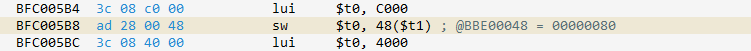
\includegraphics[width=1\textwidth]{GenDbg_GUI_Qt_Vue_code_Instruction_ecriture_memoire}};

		\draw[->,thick,green] (i3) -- ($(img.north west)+(240,-13)$);

		\draw[thick,green] (340,-40) rectangle (440,-90);
		\node[anchor=west] (capstonelogo) at (375,-32) {
\includegraphics[height=12pt]{logos/capstone.png}};
		\node[anchor=west, xshift=-5] (capstonetxt) at (capstonelogo.east) {Capstone};
	\end{tikzpicture}
\end{document}
